In this project, we proceeded in two phases. First, we explored Gem5's capabilities and developed a deeper understanding of the simulator's internal workings. To do this, we studied the impact of different instruction set architectures (ISAs) on execution speed and cache miss rates under a given workload. We used the Gem5 simulator to run a set of benchmarks and collected data on execution time and cache performance. This data was then analyzed to evaluate how different ISAs influence performance. The insights gained helped us identify the strengths and limitations of each ISA in various scenarios.

In the second phase, we worked on extending Gem5 to support the AVR architecture. We began by familiarizing ourselves with the existing codebase and identifying the components that required modification. We then implemented support for basic AVR instructions such as \texttt{add} and \texttt{sub}.

\subsection{Testing the gem5 simulator}
For the testing we used the algorithm of multiplying two matrices in row major format. The algorithm was written in C and compiled for different architectures.

\subsubsection{\textbf{Workload Compilation}} The used code was:
\begin{lstlisting}[language=C, caption={Row major matrix multiplication algorithm}, label={lst:matrix_mult}]
// Multiplication of two matrices
#include <stdio.h>
#include <stdlib.h>
#include <time.h>

int** createRandomMatrix(int n) {
    int** matrix = malloc(n * sizeof(int*));
    for (int i = 0; i < n; i++) {
        matrix[i] = malloc(n * sizeof(int));
        for (int j = 0; j < n; j++) {
            matrix[i][j] = (rand()%2==1?-1:1)*rand() % MAX; // capping the values
        }
    }
    return matrix;
}

int** createZeroMatrix(int n) {
    int** matrix = malloc(n * sizeof(int*));
    for (int i = 0; i < n; i++) {
        matrix[i] = calloc(n, sizeof(int));
    }
    return matrix;
}

void printMatrix(int** matrix, int n) {
    for (int i = 0; i < n; i++) {
        for (int j = 0; j < n; j++) {
            printf("%3d ", matrix[i][j]);
        }
        printf("\n");
    }
}

void multiplyMatrices(int** A, int** B, int** C, int n) {
    for (int i = 0; i < n; i++) {           // Row of A
        for (int j = 0; j < n; j++) {       // Column of B
            for (int k = 0; k < n; k++) {   // Iterate over row-col
                C[i][j] += A[i][k] * B[k][j];
            }
        }
    }
}

void freeMatrix(int** matrix, int n) {
    for (int i = 0; i < n; i++)
        free(matrix[i]);
    free(matrix);
}

int main() {
    int n = DIM;
    srand(time(NULL)); 

    int** A = createRandomMatrix(n);
    int** B = createRandomMatrix(n);
    int** C = createZeroMatrix(n);

    printf("Matrix A:\n");
    printMatrix(A, n);

    printf("\nMatrix B:\n");
    printMatrix(B, n);

    multiplyMatrices(A, B, C, n);

    printf("\nMatrix A x B:\n");
    printMatrix(C, n);

    freeMatrix(A, n);
    freeMatrix(B, n);
    freeMatrix(C, n);

    return 0;
}

\end{lstlisting}

The used code was compiled with two constants \texttt{DIM} and \texttt{MAX}. The constant \texttt{DIM} is the size of the matrix and the constant \texttt{MAX} is the maximum absolute value of the elements in the matrix. The code was compiled with the following command:

\begin{lstlisting}[language=bash , caption={Compilation Command}, label={lst:compilation}]
    <compiler> -static -o matrix_mult matrix_mult.c -DDIM=<dimension> -DMAX=<max_value>
\end{lstlisting}


The code was compiled with the \texttt{-static} flag to ensure that the code is statically linked. This is important because the gem5 simulator does not support dynamic linking. The code was compiled with the \texttt{-D} flag to define the constants \texttt{DIM} and \texttt{MAX}.

The code generates two random matrices of size \texttt{DIM} and multiplies them. The result is printed to the standard output. The code was compiled for the following architectures:

\begin{table}[h!]
	\centering
	\begin{tabular}{|c|c|c|}
		\hline
		\textbf{Architecture} & \textbf{Compiler}     \\
		\hline
		x86                   & gcc                   \\
		ARM                   & aarch64-linux-gnu-gcc \\
		RISCV                 & riscv-linux-gnu-gcc   \\
		\hline
	\end{tabular}
	\vspace{0.2cm}
	\caption{List of architectures and their compilers}
\end{table}

\subsubsection{\textbf{Simulation System Design}} The gem5 simulation has a modular design. It closely resembles a real system. The main part on which simulation run is a board. There are multiple types of boards in gem5. A board holds different components of a system namely clock, processor and memory. The binary resource is also loaded to this board.

\begin{lstlisting}[language=python, caption={Creating System Configuration for GEM5 simulation}, label={lst:gem5_processor}]
processor = SimpleProcessor(
    cpu_type=CPUTypes.TIMING,
    num_cores=1,
    isa=isa
)

memory = SingleChannelDDR3_1600("1GiB")

'''
Cache hierarchy can be defined in multiple ways.
For example, you can use a NoCache or a PrivateL1PrivateL2CacheHierarchy.
'''
cache_hierarchy = NoCache()

# or

cache_hierarchy = PrivateL1PrivateL2CacheHierarchy(
    l1d_size="32kB",
    l1i_size="32kB",
    l2_size="128kB"
)

board = SimpleBoard(
    clk_freq="1GHz",
    processor=processor,
    memory=memory,
    cache_hierarchy=cache_hierarchy
)

binary = BinaryResource("<path_to_binary>")
board.set_se_binary_workload(binary)

simulator = Simulator(board=board)
simulator.run()
\end{lstlisting}

The code in the listing \ref{lst:gem5_processor} shows how to create a system configuration for gem5 simulation. The code creates a simple board with a single core processor, memory and cache hierarchy. The binary resource is loaded to the board. The simulator is then run.
The code is written in Python. The gem5 simulator provides a Python API to create the system configuration. The code can be run with the following command:
\begin{lstlisting}[language=bash, caption={Running the simulation}, label={lst:gem5_run}]
./build/ALL/gem5.opt <path_to_script>
\end{lstlisting}
The code can be run with the \texttt{gem5.opt} binary. The \texttt{gem5.opt} binary is the optimized version of the gem5 simulator. The \texttt{gem5.debug} binary is the debug version of the gem5 simulator.

The simulation produces the results in \texttt{m5out} directory. The directory contains system configuration diagram and statistics.
\begin{figure}[h]
	\centering
	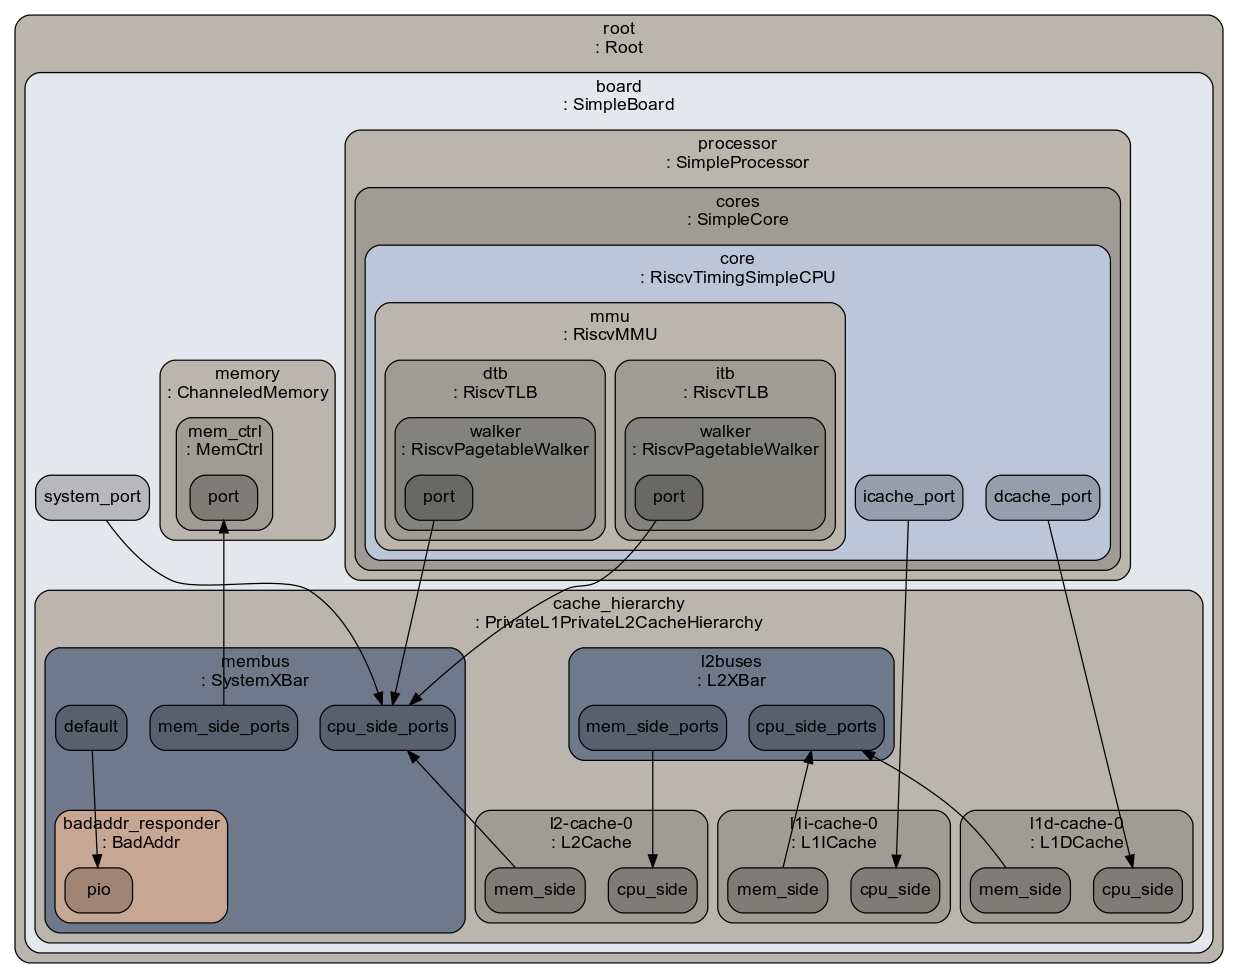
\includegraphics[width=8.5cm]{figs/config.dot.png}
	\caption{Sample System Configuration Diagram}
	\label{fig:system_config}
\end{figure}
The results are written to \texttt{stats.txt} file.

\begin{lstlisting}[language=python, caption={Sample Statistics}, label={lst:gem5_stats}]

---------- Begin Simulation Statistics ----------
simSeconds                                   0.000282                       # Number of seconds simulated (Second)
simTicks                                    281722000                       # Number of ticks simulated (Tick)
finalTick                                   281722000                       # Number of ticks from beginning of simulation (restored from checkpoints and never reset) (Tick)
simFreq                                  1000000000000                       # The number of ticks per simulated second ((Tick/Second))
hostSeconds                                      0.19                       # Real time elapsed on the host (Second)
hostTickRate                               1498170641                       # The number of ticks simulated per host second (ticks/s) ((Tick/Second))
hostMemory                                    4448164                       # Number of bytes of host memory used (Byte)
simInsts                                       172171                       # Number of instructions simulated (Count)
simOps                                         192213                       # Number of ops (including micro ops) simulated (Count)
hostInstRate                                   915165                       # Simulator instruction rate (inst/s) ((Count/Second))
                            ...
\end{lstlisting}

\subsubsection{\textbf{Simulation Parameters}} For the study of the gem5's simulation system,  we used following input parameters:
\begin{table}[ht]
	\centering
	\renewcommand{\arraystretch}{1.5} % Adjust for better vertical spacing
	\begin{tabularx}{7cm}{|>{\centering\arraybackslash}m{1.5cm}|>{\centering\arraybackslash}m{1.5cm}|>{\centering\arraybackslash}m{2.7cm}|}
		\hline
		\textbf{Parameters} & \textbf{Values}        & \textbf{Description}                                     \\
		\hline
		Architecture        & ARM, RISC-V, x86       & Instruction Set Architecture type used in the simulation \\
		\hline
		Cache Availability  & Yes, No                & Whether cache memory is available in the simulation      \\
		\hline
		L1D Size            & 32, 64, 128 kB         & Size of Level 1 data cache                               \\
		\hline
		L1I Size            & 32, 64, 128 kB         & Size of Level 1 instruction cache                        \\
		\hline
		L2 Size             & 128, 256, 512, 1024 kB & Size of Level 2 cache                                    \\
		\hline
		Matrix Dimension    & 5, 10, 20, 40, 80      & Dimension of the square matrix for multiplication        \\
		\hline
		max_val             & $10^6$                 & Maximum absolute value of the elements in the matrix     \\
		\hline
	\end{tabularx}
	\vspace{0.2cm}
	\caption{Parameters of Simulation}
	\label{tab:sim_params}
\end{table}

We restricted our study to execution speed and cache miss rates. Based on the objective we decided following target parameters to monitor: \\

\begin{table*}[t]
	\centering
	\renewcommand{\arraystretch}{1.2}
	\small
	\begin{tabularx}{\textwidth}{|>{\ttfamily}l|X|}
		\hline
		\textbf{Parameter}              & \textbf{Description}                                 \\
		\hline
		\multicolumn{2}{|l|}{\textbf{Simulation Metrics}}                                      \\
		\hline
		simSeconds                      & Simulation time in seconds                           \\
		\hline
		simTicks                        & Simulated ticks                                      \\
		\hline
		simInsts                        & Number of instructions simulated                     \\
		\hline
		simOps                          & Number of operations simulated (including micro-ops) \\
		\hline
		core.cpi                        & Cycles per instruction                               \\
		\hline
		core.ipc                        & Instructions per cycle                               \\
		\hline
		\multicolumn{2}{|l|}{\textbf{L1 Data Cache}}                                           \\
		\hline
		l1d-cache-0.demandHits::total   & Total hits to L1 data cache                          \\
		\hline
		l1d-cache-0.demandMisses::total & Total misses to L1 data cache                        \\
		\hline
		\multicolumn{2}{|l|}{\textbf{L1 Instruction Cache}}                                    \\
		\hline
		l1i-cache-0.demandHits::total   & Total hits to L1 instruction cache                   \\
		\hline
		l1i-cache-0.demandMisses::total & Total misses to L1 instruction cache                 \\
		\hline
		\multicolumn{2}{|l|}{\textbf{L2 Cache}}                                                \\
		\hline
		l2-cache-0.demandHits::total    & Total hits to L2 cache                               \\
		\hline
		l2-cache-0.demandMisses::total  & Total misses to L2 cache                             \\
		\hline
	\end{tabularx}
	\vspace{0.1cm}
	\caption{Target parameters to be monitored}
	\label{tab:monitored_params}
\end{table*}


Based on the above input parameters we simulated on \textbf{555} different configurations. The results were collected and analyzed. The results are presented in the next section.

\subsubsection{\textbf{Gem5 Extensions}}
After the study of the gem5 simulator, we worked on extending the gem5 simulator to support the AVR architecture. The AVR architecture is a RISC architecture with a simple instruction set. The AVR architecture has a 16-bit instruction set and a 32-bit data bus. The AVR architecture has a Harvard architecture with separate instruction and data memory. The AVR architecture has a 16-bit program counter and a 16-bit stack pointer. The AVR architecture has a 16-bit general purpose register file with 32 registers. The AVR architecture has a 16-bit ALU with support for arithmetic, logical and bitwise operations.

\begin{figure}[h]
	\centering
	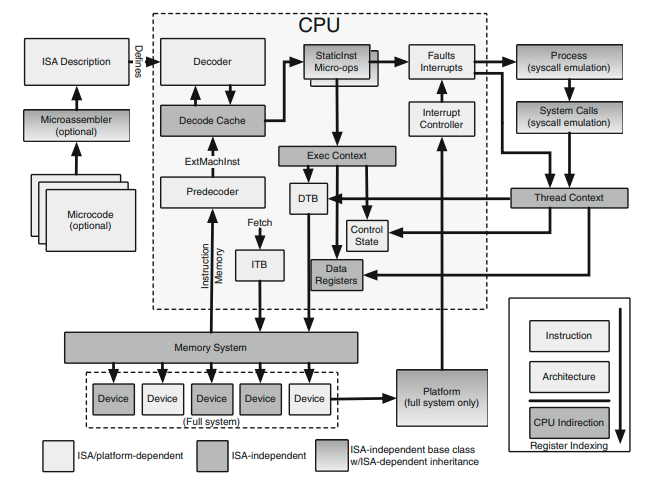
\includegraphics[width=8.5cm]{figs/impl.png}
	\caption{ISA dependency of CPU components}
	\label{fig:isa_dependence}
\end{figure}

To implement the AVR architecture in gem5, we need to implement the following major components:
\begin{itemize}
	\item \textbf{Instruction Set Architecture (ISA)}: The ISA defines the instruction set of the architecture, including:
	      \begin{itemize}
		      \item Arithmetic Logic Unit (ALU) operations (ADD, SUB, AND, OR, etc.)
		      \item Data transfer instructions (MOV, LD, ST)
		      \item Control flow instructions (RJMP, RCALL, RET)
		      \item Bit manipulation instructions (BSET, BCLR, BST, BLD)
	      \end{itemize}

	\item \textbf{Processor Core}: The processor implementation requires:
	      \begin{itemize}
		      \item 32 general-purpose 8-bit registers (R0-R31)
		      \item Program Counter (PC) and Stack Pointer (SP) implementation
		      \item Pipeline stages (fetch, decode, execute, memory, write-back)
		      \item Status Register (SREG) for flags (Zero, Carry, Overflow, etc.)
	      \end{itemize}

	\item \textbf{Memory System}: The AVR memory architecture includes:
	      \begin{itemize}
		      \item Harvard architecture with separate address spaces for program and data
		      \item Three-level memory hierarchy (registers, SRAM, and flash memory)
		      \item Memory-mapped I/O for peripheral access
		      \item EEPROM emulation for non-volatile storage
	      \end{itemize}

	\item \textbf{Peripherals}: Essential peripherals to implement:
	      \begin{itemize}
		      \item Timers/Counters (8-bit and 16-bit)
		      \item Analog-to-Digital Converter (ADC)
		      \item Universal Synchronous / Asynchronous Receiver / Transmitter (USART)
		      \item Interrupt controller for handling 35+ interrupt vectors
	      \end{itemize}
\end{itemize}

We have currently implemented the \texttt{add} and \texttt{sub} instructions. We start by defining \texttt{AVR} class derived from \texttt{SimObjects} class. To implement the instructions, we have to follow the DSL of gem5. The flow of the implementation is as follows:
\begin{figure}[h]
	\centering
	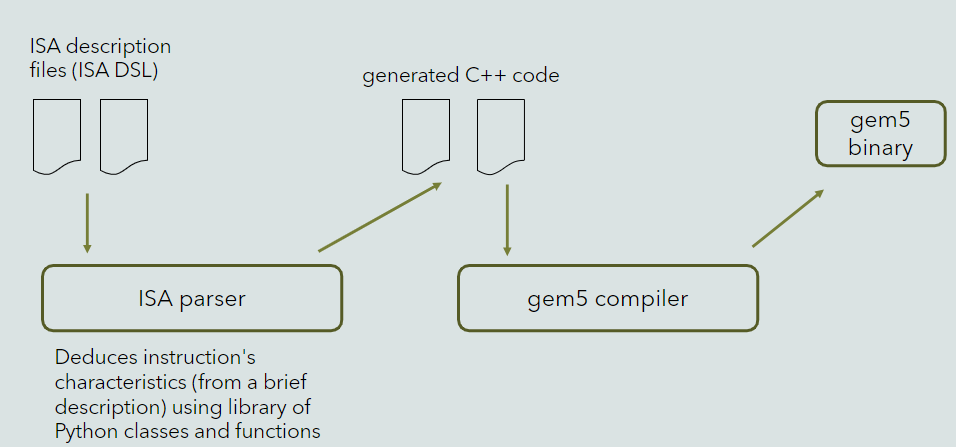
\includegraphics[width=8.5cm]{figs/flow.png}
	\caption{ISA implementation flow}
	\label{fig:implementation_flow}
\end{figure}

The build system of gem5 is based on SCons. The SCons build system is a software construction tool that uses Python scripts to define the build process. The SCons build system is used to build the gem5 simulator and its components. The SCons build system is used to generate the ISA decoder and the instruction set architecture.
\begin{lstlisting}[language=python, caption={Build script in SCons}, label={lst:scons}]
    # -*- mode:python -*-

    Import('*')
    
    DebugFlag('AVR')
    DebugFlag('AVRInst')
    DebugFlag('AVRDecoder')
    
    Source('utility.cc')
    Source('registers.cc')
    Source('faults.cc')
    Source('isa.cc')
    
    
    SimObject('AVR.py', sim_objects=['AVR'])
    
    # Generate ISA decoder
    isa_desc = ISADesc('isa/main.isa')    
\end{lstlisting}
Listing~\ref{lst:scons} shows the SCons build script for the AVR architecture. AVR features are defined across multiple \texttt{.cc} and \texttt{.hh} files. The \texttt{AVR.py} file is the main entry point for the AVR architecture. The \texttt{isa/main.isa} file contains the instruction set description for the AVR architecture. The \texttt{ISADesc} class is used to generate the ISA decoder and the instruction set architecture. The \texttt{DebugFlag} function is used to enable debugging for the AVR architecture.

Going through the implementation of the \texttt{add} instruction, we start by defining the instruction in the \texttt{isa/main.isa} file. It contains the \texttt{bitfield} definition of the instruction. The bitfield definition is used to decode the instruction.

\begin{lstlisting}[language=python, caption={Bitfield definition of the instruction}, label={lst:bitfield}]
def bitfield OPCODE    <15:10>;
def bitfield REG_D     <8:4>;
def bitfield REG_R     <3:0>;
def bitfield IMM8      <7:0>;
\end{lstlisting}

Later operands are defined in the \texttt{isa/operands.isa} file. The operands are used to define the operands of the instruction. The format of \texttt{add} instruction is as follows:
\begin{lstlisting}[language=python, caption={Operands of the instruction}, label={lst:operands}]
def format Add(code, *opt_args) {{
    iop = InstObjParams(name, Name, 'AddOp',
                        {'code': code,
                        'predicate_test': predicateTest,
                        'op_class': 'gem5::enums::IntAlu'
                        },
                        opt_args)
    header_output = AddDeclare.subst(iop)
    decoder_output = AddConstructor.subst(iop)
    decode_block = AddDecode.subst(iop)
    exec_output = AddExecute.subst(iop)
    disasm_output = AddDisassembly.subst(iop)
}};

def template AddDeclare {{
    class %(class_name)s : public gem5::AVRISAInst::AVRStaticInst
    {
      public:
        %(class_name)s(gem5::AVRISAInst::MachInst machInst);
        Fault execute(ExecContext *, trace::InstRecord *) const override;
        std::string generateDisassembly(Addr pc,
            const loader::SymbolTable *symtab) const override;
        void advancePC(PCStateBase &pc_state) const;
    };
}};

\end{lstlisting}
This format is later used by build system to generate the instruction decoder. The functions declared in the \texttt{Add} class is defined later as:
\begin{lstlisting}[language=python, caption={Instruction decoder}, label={lst:decoder}]
def template AddConstructor {{
    %(class_name)s::%(class_name)s(gem5::AVRISAInst::MachInst machInst)
        : gem5::AVRISAInst::AVRStaticInst("add", machInst, %(op_class)s)
    {
        _numSrcRegs = 0;
        _numDestRegs = 0;

        // Source registers: Rd and Rr
        setSrcRegIdx(_numSrcRegs++,
            RegId(gem5::AVRISAInst::intRegClass, bits(machInst, 8, 4)));  // Rd
        setSrcRegIdx(_numSrcRegs++,
            RegId(gem5::AVRISAInst::intRegClass, bits(machInst, 3, 0)));  // Rr

        // Destination register: Rd
        setDestRegIdx(_numDestRegs++,
            RegId(gem5::AVRISAInst::intRegClass, bits(machInst, 8, 4)));

        // Set flags
        flags[IsInteger] = true;
    }

    void %(class_name)s::advancePC(PCStateBase &pc_state) const{
        auto &avr_pc = pc_state.as<gem5::AVRISAInst::PCState>();
        avr_pc.advance();
    }
    std::string
    %(class_name)s::generateDisassembly(Addr pc,
        const gem5::loader::SymbolTable *symtab) const
    {
        std::stringstream ss;
        ss << "add r" << (int)bits(machInst, 8, 4)
            << ", r" << (int)bits(machInst, 3, 0);
        return ss.str();
    }
}};

def template AddExecute {{
    Fault
    %(class_name)s::execute(ExecContext *xc, trace::InstRecord *traceData) const
    {
        // Read source registers
        uint8_t rd = xc->getRegOperand(this, srcRegIdx(0));  // Changed to getRegOperand
        uint8_t rr = xc->getRegOperand(this, srcRegIdx(1));  // Changed to getRegOperand
        uint8_t result = rd + rr;

        // Read SREG
        uint8_t sreg = xc->readMiscRegOperand(this, AVRISAInst::MISCREG_SREG);

        // Update flags
        AVRISAInst::updateFlagsAdd(sreg, result, rd, rr);

        // Write results
        xc->setRegOperand(this, destRegIdx(0), result);  // Changed to setRegOperand
        xc->setMiscRegOperand(this, AVRISAInst::MISCREG_SREG, sreg);

        auto pc = xc->pcState().as<gem5::AVRISAInst::PCState>();
        pc.advance();
        xc->pcState(pc);

        return NoFault;
    }
}};

def template AddDisassembly {{
    std::string
    %(class_name)s::generateDisassembly(Addr pc,
        const gem5::loader::SymbolTable *symtab) const
    {
        std::stringstream ss;
        ss << "add r" << (int)bits(machInst, 8, 4)
            << ", r" << (int)bits(machInst, 3, 0);
        return ss.str();
    }
}};

\end{lstlisting}

The code is later compiled with the SCons build system. To run the simulation, we need to implement the \texttt{AVR CPU} class. The implementation of the \texttt{AVR CPU} is still pending.